\subsection{Графики обучения}\label{subsec:learning_figures}

Для лучшего понимания процесса обучения нейронной сети необходима визуализация. История обучения нейронной сети $h$, определенная в \ref{subsec:opt_hyper}, хранит значения функции потерь $f_{loss}$  и метрики $\rho$, в качестве которой была выбрана метрика \textsl{binary\_accuracy}\cite[раздел metrics]{bib:keras}, полученные в конце каждой эпохи на выборках $D_T$ и $D_T$. Ниже представлен графики зависимости значений $f_{loss}$ и $\rho$ от номера эпохи.

\begin{figure}[h]
    \centering
    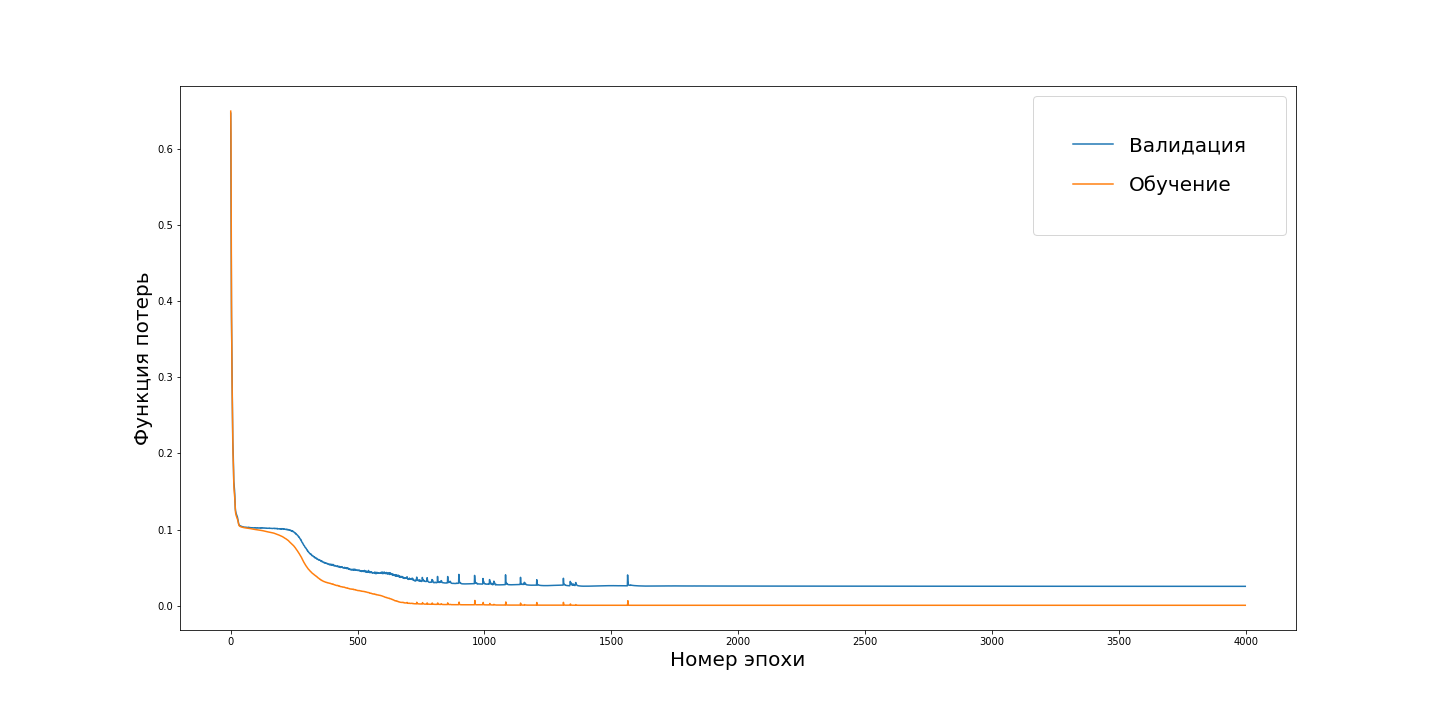
\includegraphics[scale=0.45]{model_loss}
    \caption{Функция потерь модели}
    \label{fig:loss}
\end{figure}

\newpage

\begin{figure}[h]
    \centering
    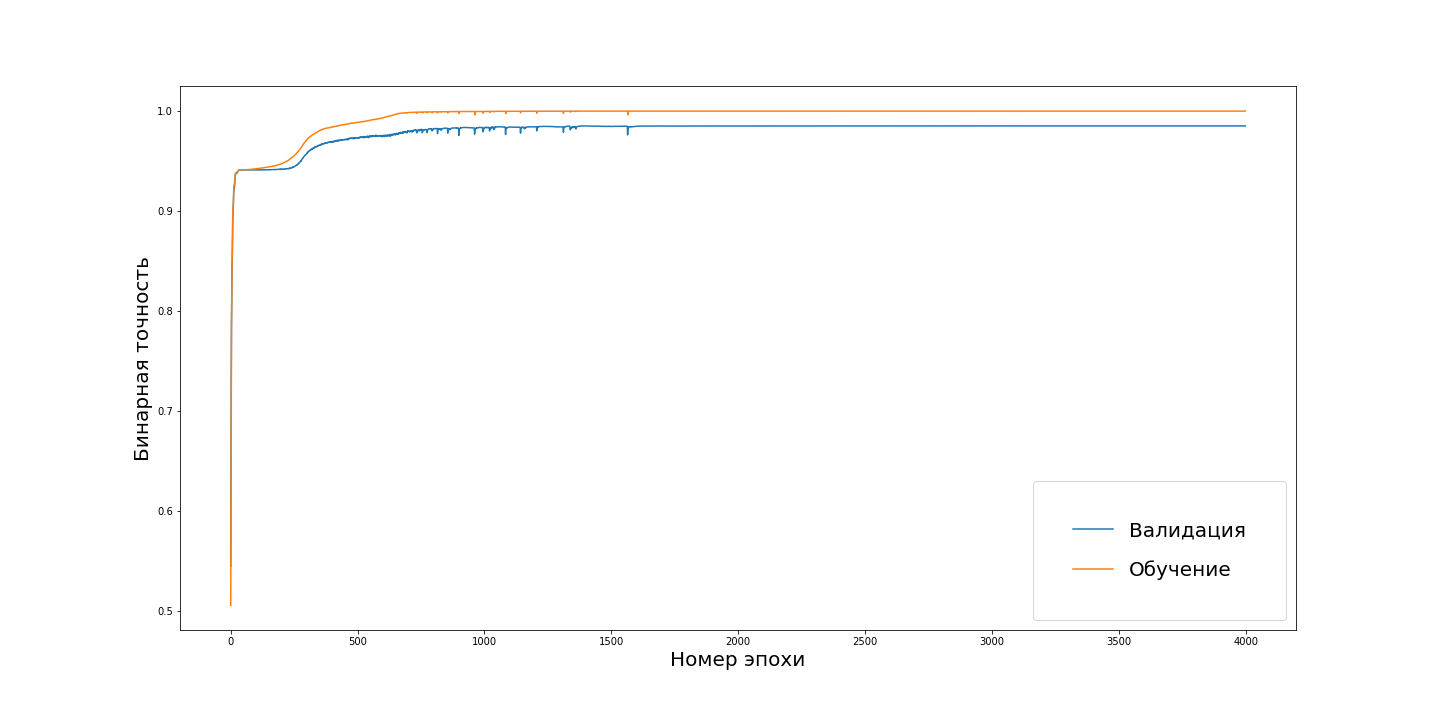
\includegraphics[scale=0.45]{model_binary_accuracy}
    \caption{Точность модели}
    \label{fig:accuracy}
\end{figure}


Из графиков видно, что после $1000$-ой эпохи $f_{loss}$ и $\rho$ практически не меняются.
